\section{Properties of the communities core}

In this section we explain about the main properties of the what we define as core communities in the previous sections.
We also show how the core community behaves in some social networks metrics and how its impacts yours communities over 
the years using temporal slide windows.

\subsection{Core over time}
Thus as the communities, the core community also evolves over the years. The Figure \ref{fig:metrics_accumulated_1_in_1}
showns how the communities evolves over the time considering data accumulated. Here, we show a different way to see the evolution,
the Figure \ref{fig:metrics_slide_window} showns the evolution of the communities over the year over the years using temporal slide 
window. It is possible to clearly see some differences, as the assortativity in Figure \ref{fig:assortativity_1_in_1}
and Figure \ref{fig:assortativity_slide_window} which in the first one, it start at 1 in many cases and stabilizes at 0 
nowadays, however, the slide windows show a large variation over the time, this may indicate, peharps, that the community come by
more variation than expected. This vision is so important to understand the core community, how we are explaing.\\
\begin{figure}[!htb]
  \begin{center}
  \subfigure[Assortativity]{%
    \label{fig:assortativity_slide_window}
    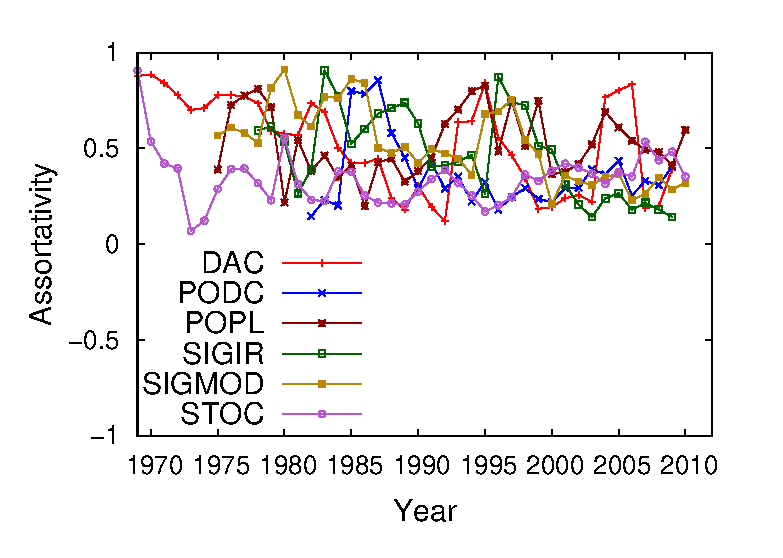
\includegraphics[scale=.33]{graficos/core_over_time/metricas_tradicionais/assortatividade_slide_window_grupo_temporal_web.eps}
  }%
  \subfigure[Average shortest path]{%
    \label{fig:average_shortest_path_slide_window}
    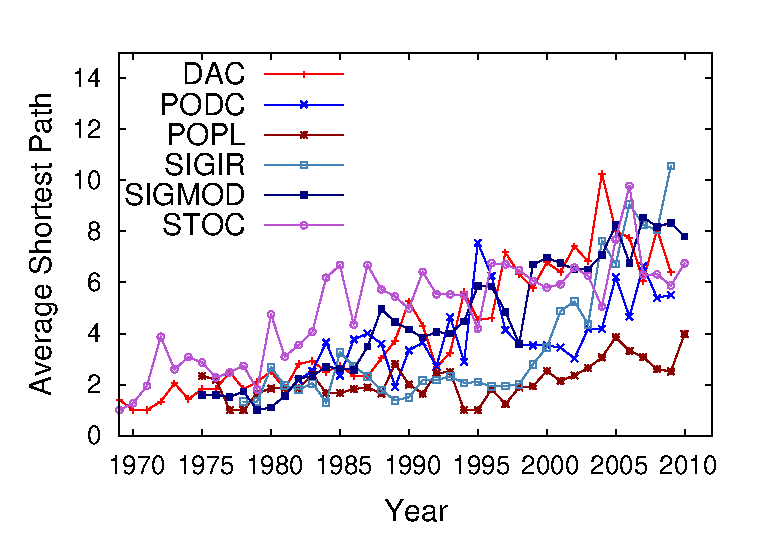
\includegraphics[scale=.33]{graficos/core_over_time/metricas_tradicionais/caminho_minimo_medio_slide_window_grupo_temporal_web.eps}
  }%
  \\
  \subfigure[Clustering coefficient]{%
    \label{fig:clustering_coefficient_slide_window}
    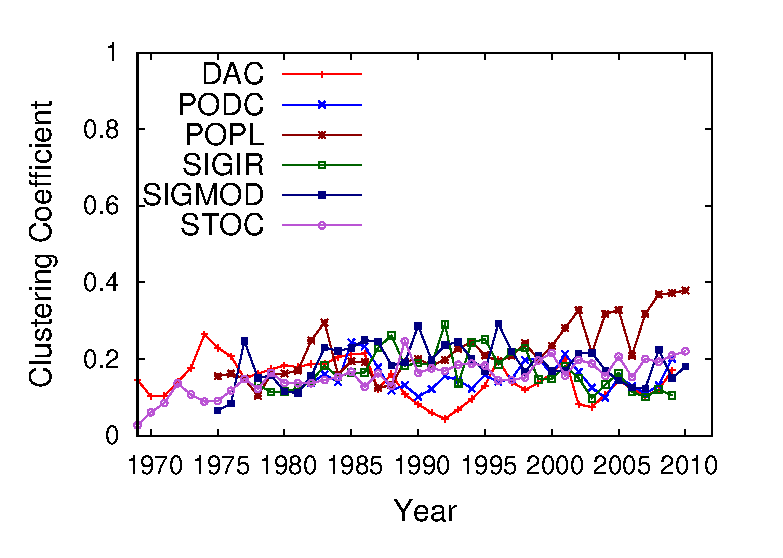
\includegraphics[scale=.33]{graficos/core_over_time/metricas_tradicionais/coeficiente_agrupamento_slide_window_grupo_temporal_web.eps}
  }%
  \subfigure[Largest connected component]{%
    \label{fig:largest_connected_component_slide_window}
    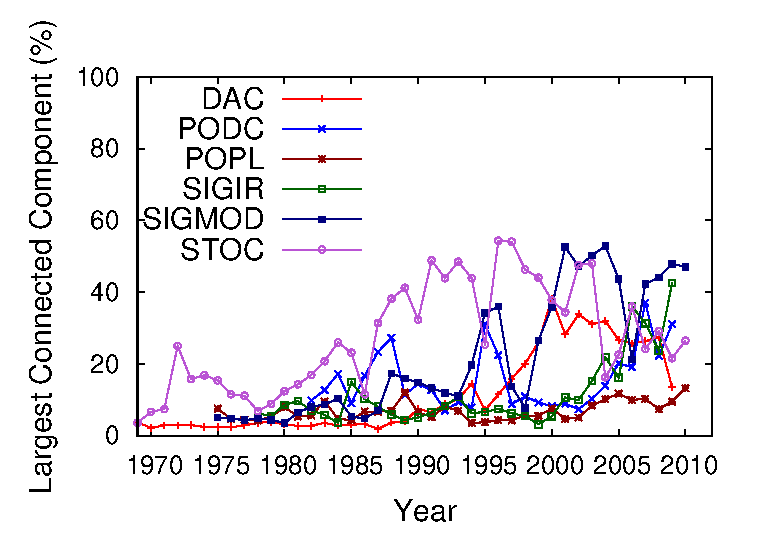
\includegraphics[scale=.33]{graficos/core_over_time/metricas_tradicionais/porcentagem_maior_componente_slide_window_grupo_temporal_web.eps}
  }%
  \\
  \subfigure[Average Degree]{%
    \label{fig:average_degree_slide_window}
    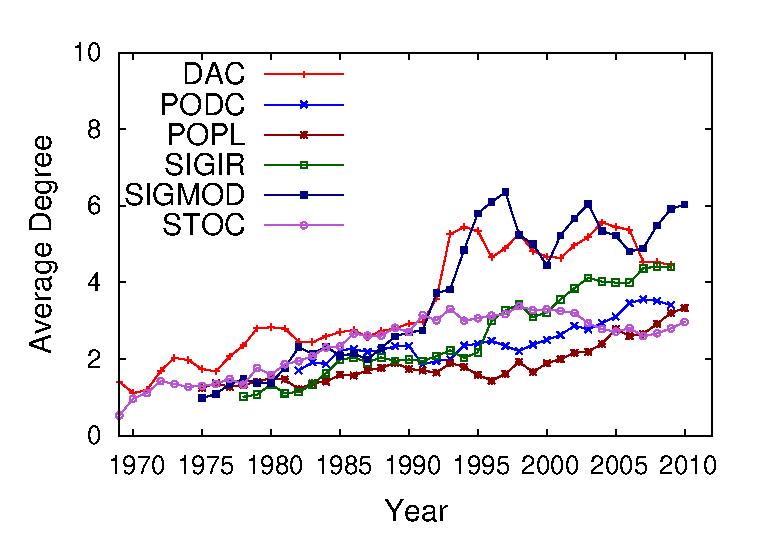
\includegraphics[scale=.33]{graficos/core_over_time/metricas_tradicionais/grau_medio_nodos_slide_window_grupo_temporal_web.eps}
  }%
  \end{center}
  \caption{Metrics using slide window of the 3 size}
  \label{fig:metrics_slide_window}
\end{figure}

In our studies about the core communities, we used the slide windows to understand how the core communities evolve. It is important
understand how the core community is clustered, because a core community very clustered may indicate a strong impact in the network.
The Figure \ref{fig:core_com_sigir_clustering_coefficient} and \ref{fig:core_com_sigmod_clustering_coefficient} shows the clustering 
coefficient of the SIGIR and SIGMOD, respectively. It is possible to see the behavior of the conference and the core community, the
two values are always so close, indicating that the core community has well clustering relative the conference.\\

\begin{figure*}[!htb]
  \begin{center}
  \subfigure[SIGIR - Clustering coefficient]{%
    \label{fig:core_com_sigir_clustering_coefficient}
    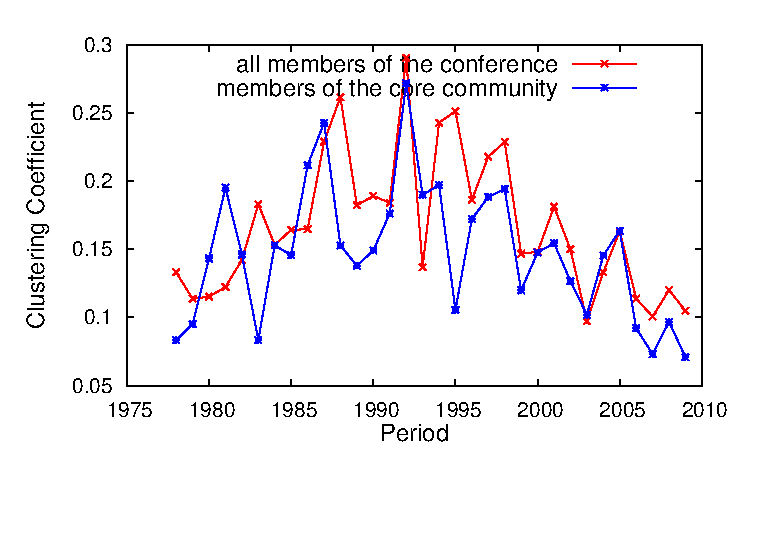
\includegraphics[scale=.33]{graficos/core_over_time/core_community/sigir_janela_3_core_coeficiente_agrupamento.eps}
  }%
  \subfigure[SIGIR - Average Degree]{%
    \label{fig:core_com_sigir_average_degree}
    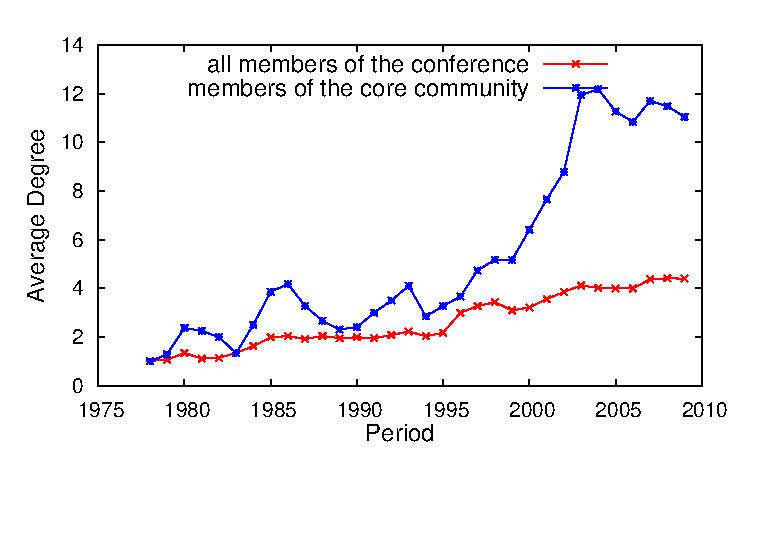
\includegraphics[scale=.33]{graficos/core_over_time/core_community/sigir_janela_3_core_grau_medio_nodos.eps}
  }%
  \subfigure[SIGIR - Largest connected component]{%
    \label{fig:core_com_sigir_largest_connected_component}
    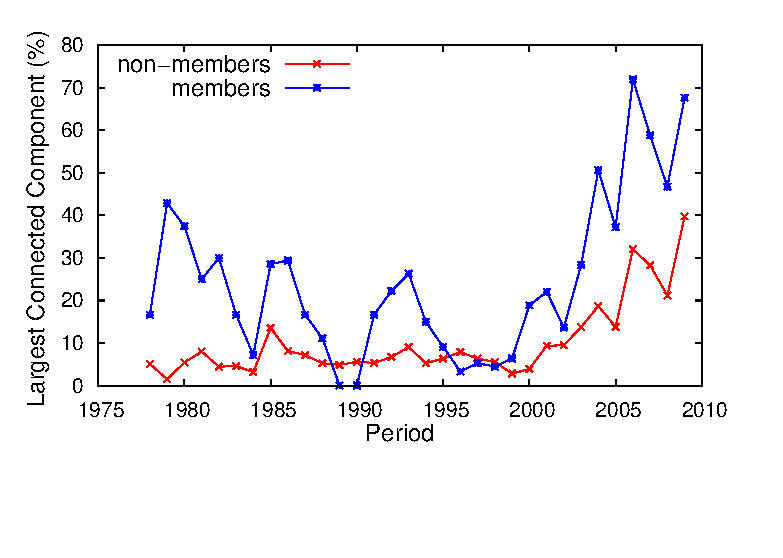
\includegraphics[scale=.33]{graficos/core_over_time/core_community/sigir_janela_3_core_maior_componente_conectado.eps}
  }%
  \\
  \subfigure[SIGMOD - Clustering coefficient]{%
    \label{fig:core_com_sigmod_clustering_coefficient}
    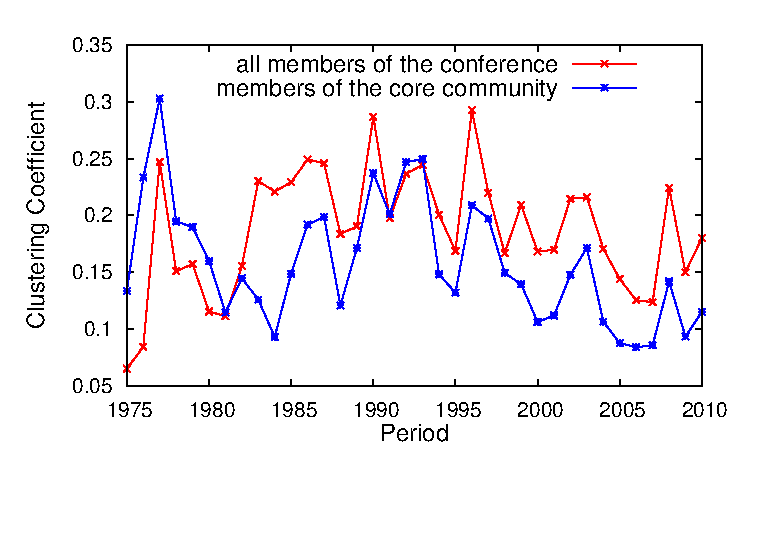
\includegraphics[scale=.33]{graficos/core_over_time/core_community/sigmod_janela_3_core_coeficiente_agrupamento.eps}
  }%
  \subfigure[SIGMOD - Average Degree]{%
    \label{fig:core_com_sigmod_average_degree}
    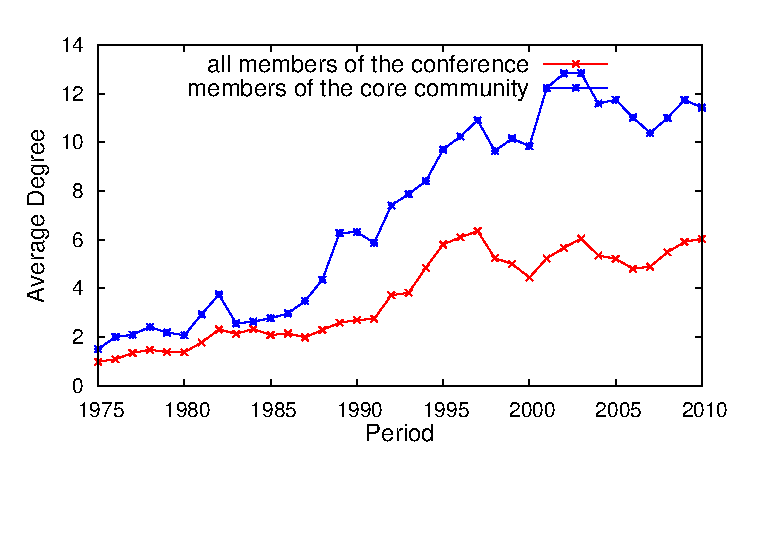
\includegraphics[scale=.33]{graficos/core_over_time/core_community/sigmod_janela_3_core_grau_medio_nodos.eps}
  }%
  \subfigure[SIGMOD - Largest connected component]{%
    \label{fig:core_com_sigmod_largest_connected_component}
    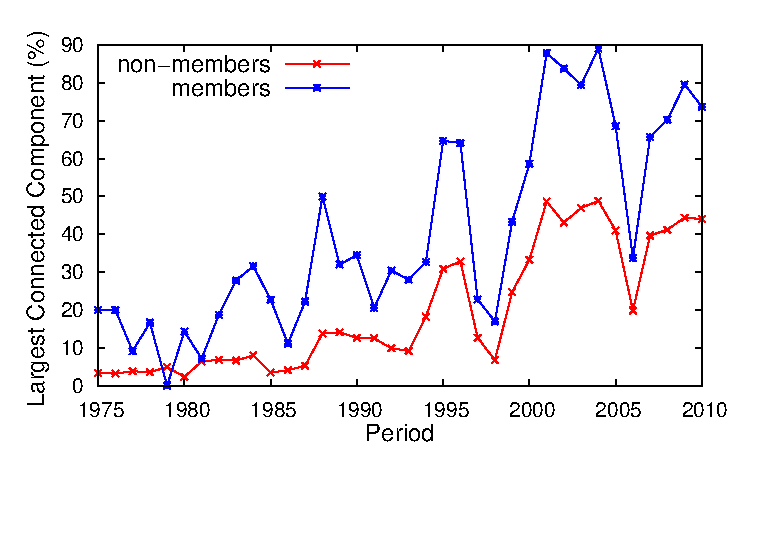
\includegraphics[scale=.33]{graficos/core_over_time/core_community/sigmod_janela_3_core_maior_componente_conectado.eps}
  }%
  \end{center}
  \caption{Metrics comparing the core community}
  \label{fig:metrics_comparing_core_community}
\end{figure*}

Over the years, a normal process is the researchers creates many links to another researchers, as students either or researchers of same 
institution or others physical places. The link to other researchers can be motivated by financial incetives the government, for exemple.
This scenario, the behavior of the links, can be seen in the Figure \ref{fig:core_com_sigir_average_degree} and 
\ref{fig:core_com_sigmod_average_degree}, it is important to note which this study do not use accumulated data, so the degree nodes of
the core community are always, generally, increasing over the years, reaching values higher than the community itself.\\
The core communities have the more important researchers in the network, in order, it is intuitive which many members of the core community
should be inside the largest connected component of the network, however, the Figure \ref{fig:core_com_sigir_largest_connected_component} and 
\ref{fig:core_com_sigmod_largest_connected_component} shows that this intuition is not totally correct, since in some periods the value of the
members of the core community into the largest connected component is 0.



\subsection{Average Community Core}

\begin{figure}[!htb]
\centering
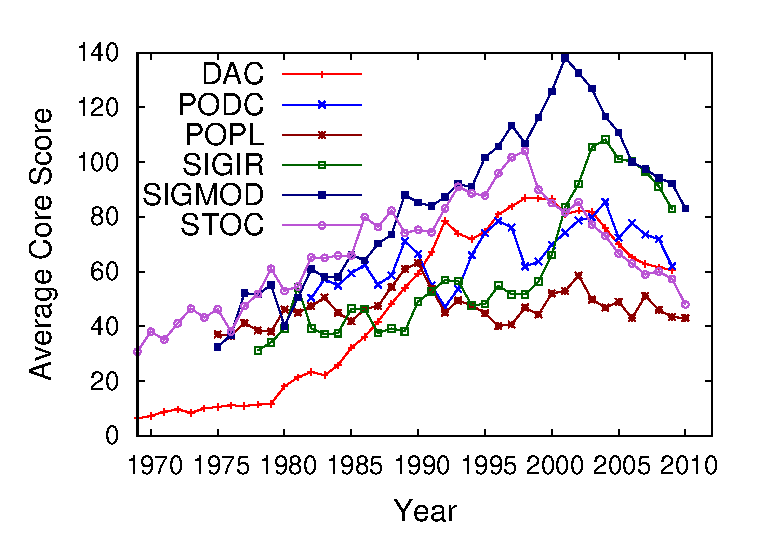
\includegraphics[scale=.5]{graficos/average_core_score/average_core_score_slide_window_grupo_temporal_web.eps}
\caption{Average Core Score}
\label{fig:average_core_score}
\end{figure}

\subsection{Core communities and Network Structure}
{\bf reproduzir trabalho do rich club \cite{Xu:2010}}

We now examine to what extent the community core fluctuations affect the network structure.


\begin{table*}[!htb]
\centering
\caption{Corelation between average core score of the core community and the metrics of complex networks}
\label{tab:correlation_metrics}
{\small
\begin{tabular}{|l|c|c|c|c|c|c|c|} \hline
Conference & Diameter & Ave. Short P. & Clus. Coef. & Assort. & Larg. Com. Con. & Ave. Deg. Node & Num. Nodes\\ \hline
CCS & 0,34 & 0,2 & 0,23 & -0,2 & 0,45 & 0,14 & -0,13\\ \hline
CHI & 0,75 & 0,79 & -0,62 & -0,74 & 0,76 & 0,77 & 0,58\\ \hline
CIKM & 0,56 & 0,56 & -0,52 & -0,67 & 0,39 & 0,87 & 0,64\\ \hline
DAC & 0,8 & 0,85 & -0,49 & -0,63 & 0,76 & 0,92 & 0,84\\ \hline
HSCC & 0,17 & 0,45 & -0,62 & -0,71 & 0,87 & 0,55 & -0,55\\ \hline
ICSE & 0,81 & 0,83 & -0,52 & -0,84 & 0,68 & 0,8 & 0,78\\ \hline
ISCA & 0,63 & 0,55 & 0,54 & -0,32 & 0,63 & 0,81 & 0,41\\ \hline
ISSAC & 0,05 & 0,01 & -0,25 & -0,43 & -0,07 & 0,21 & 0,78\\ \hline
KDD & 0,1 & 0,17 & -0,33 & -0,67 & 0,2 & 0,14 & 0,2\\ \hline
MICRO & 0,35 & 0,35 & 0,28 & -0,36 & 0,52 & 0,51 & 0,36\\ \hline
MOBICOM & -0,04 & 0,11 & 0,13 & -0,65 & 0,23 & -0,09 & 0,02\\ \hline
Multimedia & 0,67 & 0,68 & -0,91 & -0,95 & 0,67 & 0,69 & 0,75\\ \hline
PODC & 0,4 & 0,42 & -0,23 & -0,2 & 0,13 & 0,68 & 0,57\\ \hline
POPL & 0,21 & 0,2 & 0,23 & -0,43 & 0,25 & 0,19 & 0,05\\ \hline
SAC & 0,48 & 0,59 & 0,16 & -0,39 & -0,55 & 0,16 & 0,23\\ \hline
SIGCOMM & 0,18 & 0,19 & 0,05 & -0,81 & 0,49 & 0,41 & -0,03\\ \hline
SIGCSE & 0,88 & 0,84 & -0,22 & -0,5 & 0,93 & 0,87 & 0,8\\ \hline
SIGDOC & 0,73 & 0,78 & -0,36 & -0,89 & 0,66 & 0,76 & 0,05\\ \hline
SIGGRAPH & 0,79 & 0,85 & -0,45 & -0,75 & 0,94 & 0,88 & 0,55\\ \hline
SIGIR & 0,83 & 0,85 & -0,42 & -0,77 & 0,7 & 0,89 & 0,88\\ \hline
SIGMETRICS & 0,31 & 0,24 & 0,3 & -0,44 & 0,37 & 0,64 & 0,43\\ \hline
SIGMOD & 0,78 & 0,81 & 0,27 & -0,61 & 0,77 & 0,87 & 0,68\\ \hline
SIGUCCS & 0,38 & -0,22 & 0,53 & -0,13 & 0,51 & 0,7 & 0,57\\ \hline
STOC & 0,61 & 0,63 & 0,54 & -0,37 & 0,82 & 0,88 & 0,68\\ \hline
{\bf Average} & {\bf 0,49} & {\bf 0,49} & {\bf -0,11} & {\bf -0,56} & {\bf 0,5} & {\bf 0,59} & {\bf 0,42}\\ \hline
\end{tabular}
}
\end{table*}



